\section{Ejercicio}\label{ej:Chap03Ejercicio04}

El tanque de gas combustible de un automóvil equipado con GNC es de $\SI{60}{l}$. Asumiendo que el gas es metano en su totalidad, determinar la masa en $\SI{}{kg}$ que se puede almacenar a la presión de $\SI{20}{bar(a)}$ y a una temperatura de $\SI{45}{\celsius}$ utilizando un modelo de
\begin{enumerate}
    \item Gas ideal.
    \item Gas real.
\end{enumerate}
¿Cuál es la densidad del gas en estas condiciones considerando cada uno de los modelos? ¿Qué error (absoluto y relativo) se comete al aproximar con el modelo de gas ideal? ¿Es por defecto o por exceso?

En este estado, ¿el metano es líquido? Y, finalmente, ¿qué fuerza se ejerce sobre una superficie circular de $\SI{30}{cm}$ de diámetro (como podría ser una de las tapas del tubo que contiene al gas, ver figura \ref{im:Chap03-001}) bajo esa presión?

\begin{figure}[ht]
\centerline{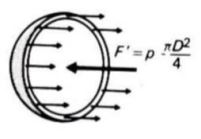
\includegraphics[scale=0.6]{001.jpg}}
\caption{\textit{La fuerza neta se obtiene con el área proyectada del casquete.}}
\label{im:Chap03-001}
\end{figure}